\mychapter{Geometria analítica plana}{Geometria analítica}{
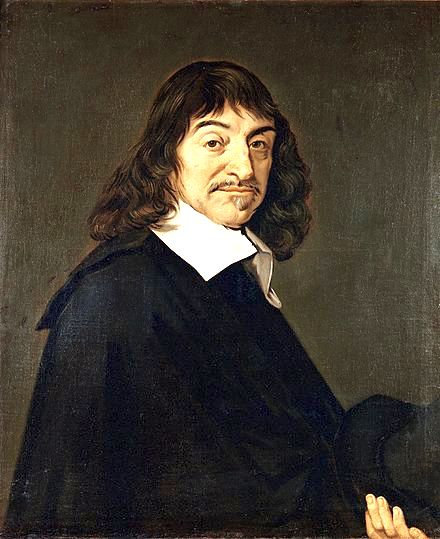
\includegraphics[width=4cm]{img-09/descartes}

{\small René Descartes (1596-1650)}
}{chap:analitica}
 

\begin{blueshaded}
	\begin{wrapfigure}{R}{0.5\textwidth}
		\begin{center}
			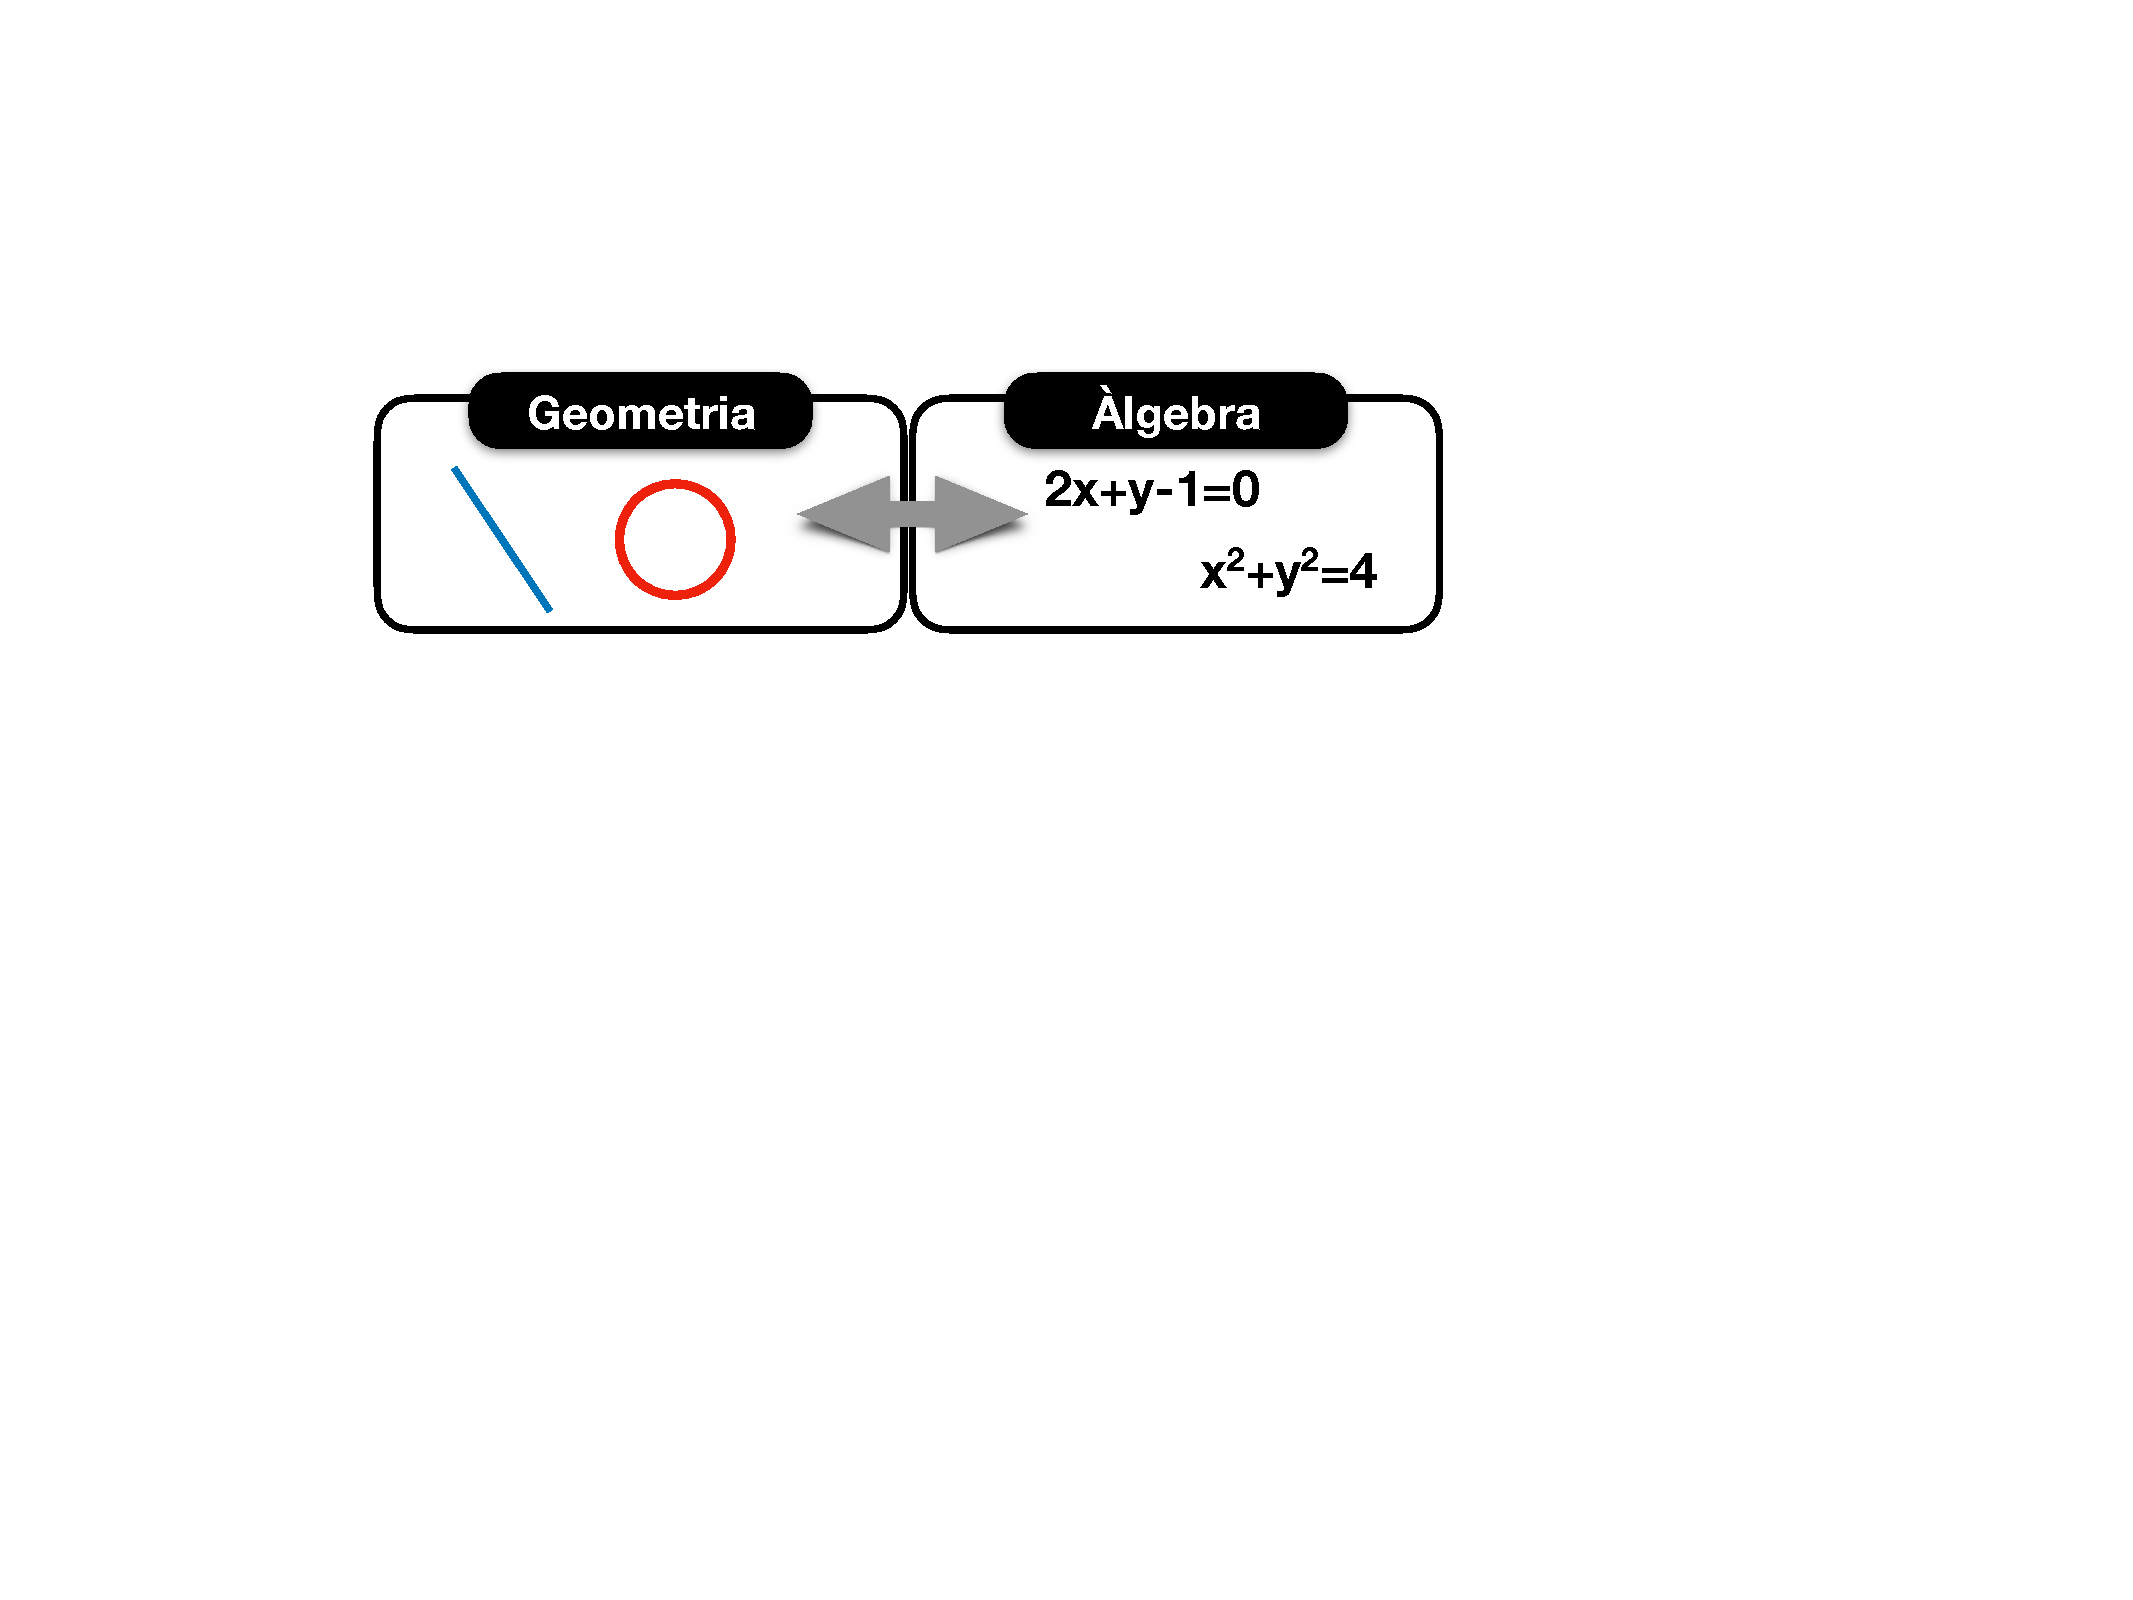
\includegraphics[width=0.4\textwidth]{img-09/analitica}
		\end{center}
	\end{wrapfigure}
	La geometria analítica permet representar figures geomètriques mitjançant fórmules.  
	Va ser inventada per René Descartes i per Pierre Fermat  a principis del segle XVII.
	A més, Descartes i Fermat van observar  que les equacions algebraiques corresponen amb figures geomètriques. Això vol dir que les línies i certes figures geomètriques es poden expressar com equacions i, al seu torn, les equacions poden dibuixar-se com línies o figures geomètriques. 	
\end{blueshaded}

\section{Punts en el pla}

\begin{theorybox}[Sistema de referència Cartesià]
	 \begin{wrapfigure}{R}{0.3\textwidth} 
		\vspace{-0.5cm}
		\begin{center}
			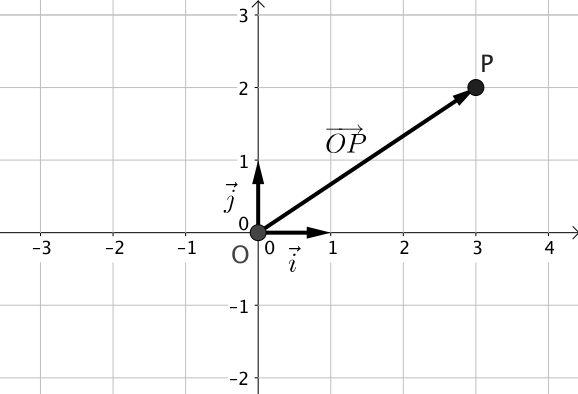
\includegraphics[width=0.28\textwidth]{img-09/cartesian}
		\end{center}
	\end{wrapfigure}
	Per localitzar punts en el pla utilitzam un sistema de referencia Cartesià (en honor a René Descartes) format per:
	\begin{itemize}
		\item Un punt $O$ anomenat origen
		\item Una base de vectors ortonormals $\vec i$, $\vec j$
	\end{itemize}
	Qualsevol punt $P$ queda determinat mitjançant el \textbf{vector de posició} $\overrightarrow{OP}$.
\end{theorybox}

\pagebreak

\begin{theorybox}[Punt mitjà d'un segment]
 	Les coordenades del punt mitjà, $M$, d'un segment d'extrems $A(A_x, A_y)$ i $B(B_x, B_y)$ són:
	\begin{equation}
	M=\frac{A+B}{2} \,\,\,\,\,\, o \,\,\,\,\,\, M \left( \frac{A_x+B_x}{2},  \frac{A_y+B_y}{2} \right)
	\end{equation}
	
\end{theorybox}


\begin{theorybox}[Punt simètric respecte d'un punt]
	\begin{wrapfigure}{R}{0.25\textwidth} 
		\vspace{-0.5cm}
		\begin{center}
			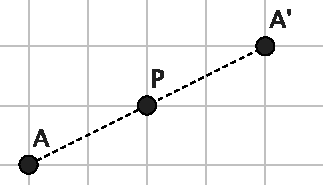
\includegraphics[width=0.23\textwidth]{img-09/simetric}
		\end{center}
	\end{wrapfigure}
	Si volem calcular el punt simètric $A'$ del punt $A$ respecte del punt $P$ raonam de la següent forma:
	El punt $P$ ha d'ésser el punt mitjà de l'interval $A'A$ amb la qual cosa es compleix que  $P = \frac{A+A'}{2}$. Si aïllam $A'$ obtenim 
	\begin{equation*}
	A' = 2P-A \,\,\,\,\,\, o \,\,\,\,\,\,A' \left( 2P_x-A_x,  2P_y-A_y \right)
	\end{equation*}
	
\end{theorybox}



\begin{theorybox}[Condició d'alineament de 3 punts]
	\begin{wrapfigure}{R}{0.3\textwidth} 
		\vspace{-1.1cm}
		\begin{center}
			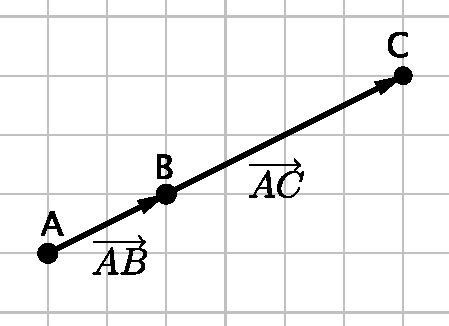
\includegraphics[width=0.28\textwidth]{img-09/alineats}
		\end{center}
	\end{wrapfigure}
	Tres punts $A(A_x, A_y)$, $B(B_x, B_y)$, $C(C_x, C_y)$ estan alineats si un parell de vectors $\overrightarrow{AB}$ i $\overrightarrow{AC}$ tenen igual direcció [Veure equació (\ref{eq:vect-align})]. En components, això passa si
	\begin{equation}
		\frac{B_x-A_x}{C_x-A_x}=\frac{B_y-A_y}{C_y-A_y}
	\end{equation}
	 
\end{theorybox}

\begin{resolt}[E]{Troba les coordenades dels punts que divideixen el segment $A(-2,5)$, $B(4,-1)$ en tres parts iguals.}
	Calculam el vector $\overrightarrow{AB}=B-A=(6,-6)$. Els punts seran:
	\vspace{0.2cm}
	
	$A+\frac{1}{3}\overrightarrow{AB}=(-2,5)+(2,-2)=(0,3)$ i
	\vspace{0.2cm}
	
	$A+\frac{2}{3}\overrightarrow{AB}=(-2,5)+(4,-4)=(2,1)$.
\end{resolt}
\begin{resolt}{Troba el punt simètric de $A(2,-1)$ respecte del punt $P(-3,5)$}
	\vspace{0.2cm}
	El simètric s'obté de $A' = 2P-A=2(-3,5)-(2,-1)=(-8, 11)$. Podeu comprovar que el punt mitjà de $A$ i $A'$ és $P$.
\end{resolt}
\begin{resolt}{Calcula el valor de $k$ perquè els punts $A(0,3)$, $B(-2, 5)$ i $C(4, k)$ estiguin alineats.}
	\vspace{0.2cm}
	Calculam els vectors $\overrightarrow{AB}=B-A=(-2, 2)$ i $\overrightarrow{AC}=C-A=(4,k-3)$. Ara imposam que aquests dos vectors tinguin igual direcció; les components han d'ésser proporcionals.
	\begin{equation*}
	\frac{-2}{4}=\frac{2}{k-3}
	\end{equation*}
	Multiplicant en creu $-2(k-3)=8$ i d'aquí trobam que $k=-1$.
\end{resolt}

\begin{mylist}
	 \exer  Donats els punts $A=\left(1,4\right)$ i $B=\left(-3,6\right)$ calcula el seu punt mitjà:
	a) Construint el vector que els uneix.
	b) Amb la fórmula. Comprova que surt el mateix.
	
	\answers{[$\overrightarrow{AB}=(-4,2)$ i $M=A+\frac{1}{2}\overrightarrow{AB}=(1,4)+(-2,1)=(-1,5)$, $M=\frac{A+B}{2}=\frac{(-2,10)}{2}=(-1,5)$]}
	
	\exer  Considera el segment d'extrems $P=\left(-2, 1 \right)$ i $Q=\left(7, 4\right)$. Calcula els punts sobre aquest segment que el divideixen en 3 parts iguals. 
	
	\answers{$\overrightarrow{PQ}=(9,3)$ i $X_1=P+\frac{1}{3}\overrightarrow{PQ}=(-2,1)+(3,1)=(1,2)$;
	$X_2=P+\frac{2}{3}\overrightarrow{PQ}=(-2,1)+(6,2)=(4,3)$.}
	
	\exer Calcula el valor de $k$ perquè els punts $A(1,7)$, $B(-3,4)$ i $C(k,5)$ estiguin alineats.
	
	\answers{$\overrightarrow{AB}=(-4,-3)$; $\overrightarrow{AC}=(k-1,-2)$; $\frac{-4}{k-1}=\frac{-3}{-2}$ $\rightarrow$ $k=-5/3$. }
	
	\exer Donats els punts $P(3,9)$ i $Q(8,-1)$ troba: a) el punt mitjà, b) el simètric de $P$ respecte  $Q$ i c) el simètric de $Q$ respecte  $P$.
 
 	\answers{[$M(\frac{11}{2},4)$, $P'(13,-11)$, $Q'(-2,19)$]}
 
	
\end{mylist}

\section{Les equacions de la recta en el pla}


\begin{theorybox}
	\videonw{189}{Equació de la recta en el pla}
	L'equació de la recta que passa pel punt $P(P_x,P_y)$ i té vector director $\vec d=(d_x, d_y)$ es pot expressar de diferents formes:
	
	\begin{minipage}{0.56\textwidth}
	\textbf{Vectorial}: $(x,y)=(P_x,P_y)+\lambda (d_x, d_y)$ \vspace{0.25cm}
	
	\textbf{Paramètriques:} $\left\{ \begin{array}{l} x=P_x+ \lambda d_x \\ y=P_y+ \lambda d_y  \end{array} \right.$\vspace{0.25cm}
	
	\textbf{Contínua:} $\dfrac{x-P_x}{d_x}=\dfrac{y-P_y}{d_y}$\vspace{0.25cm}
	\end{minipage}
	\begin{minipage}{0.4\textwidth}
		\centering
		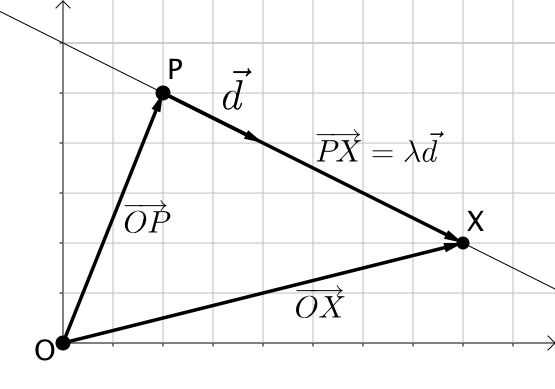
\includegraphics[width=0.9\textwidth]{img-09/rectavec}
	\end{minipage}
	\textbf{Punt-pendent:} $y-P_y=m(x-P_x)$, essent \fbox{$m=\frac{d_y}{d_x}$} el pendent de la recta.\vspace{0.25cm}
	
	\textbf{Implícita o general:} $Ax+By+C=0$, essent $(A,B)$ el vector normal de la recta. $(-B,A)$ seria un vector director.\vspace{0.25cm}
		
	
	\textbf{Explícita:} $y=mx+n$, essent $m$ el pendent i $n$ l'ordenada a l'origen.
	
\end{theorybox}

\begin{resolt}{Escriu l'equació de la recta que passa pels punts $A(3,1)$ i $B(1,4)$ de totes les formes possibles.}
	Primer calculam el vector director de la recta $\vec d = \overrightarrow{AB}=(-2,3)$ i triam un dels punts, per exemple $A$.\vspace{0.25cm}
	
	L'equació vectorial és $(x,y)=(3,1)+\lambda(-2,3)$
	
	Les paramètriques són $\left\{ \begin{array}{l} x=3-2\lambda \\ y=1+3\lambda \end{array} \right.$
	
	L'equació contínua $\frac{x-3}{-2}=\frac{y-1}{3}$
	
	La punt-pendent $y-1 = -\frac{3}{2}(x-3)$
	
	La general $3x+2y-11=0$
	
	L'explícita $y=-\frac{3}{2}x+\frac{11}{2}$
	
\end{resolt}


\begin{mylist}
	\exer Escriu l'equació de la recta que passa pel punts $A(1,-2)$ i $B(3,5)$ de totes les formes possibles.
	\answers{Vectorial: $(x,y)=(1,-2)+\lambda(2,7)$
		\par
		Paramètriques: $\left\{ \begin{array}{l} x=1+2\lambda \\ y=-2+7\lambda \end{array} \right.$
		\par
		Contínua: $\frac{x-1}{2}=\frac{y+2}{7}$
		\par
		Punt-pendent $y+2 = \frac{7}{2}(x-1)$
		\par
		General: $7x-2y-11=0$
		\par
		Explícita: $y=\frac{7}{2}x-\frac{11}{2}$}
	
	\exer Obté un punt i un vector director de cadascuna d'aquestes rectes:
	\begin{tasks}(2)
		\task $\dfrac{x}{3}=\dfrac{y+1}{-2}$
		\task $y-2=4(x+7)$
		\task $x+y-2=0$
		\task $\left\{\begin{array}{l} x=2-3\lambda \\ y=2 \end{array}\right.$		
	\end{tasks}

\answers{[$P(0,-1)$; $\vec d(3,-2)$, 
	$P(-7,2)$; $\vec d(1,4)$, 
	$P(0,2)$; $\vec d(-1,1)$, 
	$P(2,2)$; $\vec d(-3,0)$]}

	\exer Obté un punt i un vector director de la recta $y=2x+5$ i expressa-la de totes les altres formes possibles.
	
	\answers{$P(0,5)$; $\vec d(1,2)$\par
		Vectorial: $(x,y)=(0,5)+\lambda(1,2)$
		\par
		Paramètriques: $\left\{ \begin{array}{l} x=\lambda \\ y=5+2\lambda \end{array} \right.$
		\par
		Contínua: $\frac{x}{1}=\frac{y-5}{2}$
		\par
		Punt-pendent $y-5 = 2 (x-0)$
		\par
		General: $2x-y+5=0$ }
		
	\exer  Considerem la recta $r:\,  (x,y) = \left(1,3\right)+\lambda \left(1,-2\right)$.
	\begin{tasks}
		%
		\task  Calcula el seu pendent.
		%
		\task  Pertany el punt $\left(2,\, \, 2\right)$ a la recta? I el punt $\left(0,-2\right)$?
		%
		\task  Dóna almenys tres punts de la recta.
		%
		\task  Dibuixa la recta.
	\end{tasks}

\answers[cols=1]{[$\vec d=(1,-2)$; $m=-2$,
		$(2,2) \notin r$; $(2,2) \notin r$,
		$(2,1)$; $(3,-1)$; $(0,5)$, \mbox{}\par 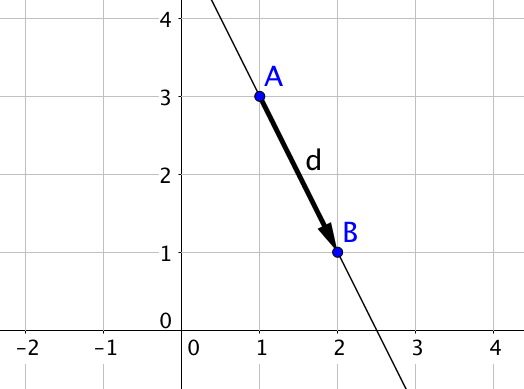
\includegraphics[width=0.4\textwidth]{img-sol/t9-8d} ]}
\end{mylist} 

%%%%%%%%%%%%%%%%%%%%%%%%%%%%%%%%%%%%%%%%%%%%%%%%%%%%%%%%%%%%%%%%%%%%%%%%%%%%%%%%%%%%%%%%%%%%%%%
\section{Recta paral·lela i perpendicular a una donada}

\begin{theorybox}[Segons vectors]
	Si ens donen una recta que té vector director $\vec d(d_x, d_y)$, per calcular
	\begin{itemize}
		\item una recta \textbf{paral·lela} a ella, utilitzam el \textbf{mateix vector} director (o proporcional).
		\item una recta \textbf{perpendicular} a ella, utilitzam el \textbf{vector normal}  $\vec n(-d_y, d_x)$.
	\end{itemize}
\end{theorybox}	

\begin{theorybox}[Segons pendents]
	Si ens donen una recta que té pendent $m$, per calcular
	\begin{itemize}
		\item una recta \textbf{paral·lela} a ella, utilitzam el \textbf{mateix pendent}.
		\item una recta \textbf{perpendicular} a ella, utilitzam el pendent $m'=-\frac{1}{m}$.
	\end{itemize}
\end{theorybox}	

\begin{resolt}[E]{Calcula l'equació general de la recta perpendicular a \[r:\, \frac{x}{-2}=\frac{y+2}{1}\] que passa pel punt $P(1,1)$}
		La recta $r$ té com a vector director $\vec d_r=(-2,1)$. El seu vector normal és $\vec n=(1,2)$. L'equació de la recta que ens demanen en forma contínua 
		\begin{equation*}
				\frac{x-1}{1}=\frac{y-1}{2}
		\end{equation*}
		Si la multiplicam en creu la passam a forma general $2x-y-1=0$.
\end{resolt}	
\begin{resolt}{Calcula l'equació general de la recta paral·lela a \[r:\, y-5=\frac{1}{2}(x+1)\] que passa per l'origen de coordenades.}
	La recta $r$ té com a pendent $m=1/2$, i la recta paral·lela tindrà el mateix pendent. L'únic que hem de fer és canviar el punt per l'origen $(0,0)$. L'equació punt-pendent serà:
	\begin{equation*}
		y-0=\frac{1}{2}(x-0)
	\end{equation*}
	Si passam a forma general trobam $x-2y=0$.
\end{resolt}

\begin{mylist}
  	

 
\exer  Calculau la recta que és paral·lela a $r$: $\frac{x-1}{2} =\frac{y-2}{3} $ i passa pel punt $P\left(0,\; 1\right)$. Expressa-la almenys en tres formes i dibuixa-les.

\answers{$\frac{x-0}{2} =\frac{y-1}{3}$; $3x-2y+2=0$; $y=\frac{3}{2}x+1$}

\exer  Calculau la recta que és paral·lela a $r$: $2x-3y=0$ i passa pel punt $P\left(1,\; 2\right)$. Expressa-la en forma contínua i dibuixa-les.
\answers{$2x-3y+C=0$ essent $C=6-2=4$; $(x,y)=(1,2)+\lambda (3,2)$; $\frac{x-1}{3}=\frac{y-2}{2}$}

 
\exer  Calculau una recta perpendicular a $r:$ $y=2x-1$ que passi per $P\left(2,\, \, -1\right)$. Expressa-la en forma paramètrica i dibuixa-la.

\answers{$y=-\frac{1}{2}x+n$ essent $n=0$; En forma paramètrica: $\left\{ \begin{array}{l} y=2-2\lambda \\ y=-1+\lambda \end{array} \right.$}

\exer D'una recta $r$ coneixem el seu pendent $m=\frac{2}{3}$. Troba la recta $s$ que es perpendicular a $r$ i que conté l'origen de coordenades.

\answers{$y=-\frac{3}{2}x$ passa per $(0,0)$}

\exer  Calculau una recta perpendicular a $r:$ $x+2y=5$ que passi per $P\left(2,\, \, 0\right)$. Troba el punt d'intersecció entre les dues rectes.
	
\answers{$t:\, 2x-y-4=0$; $X(\frac{13}{5}, \frac{6}{5})$\par 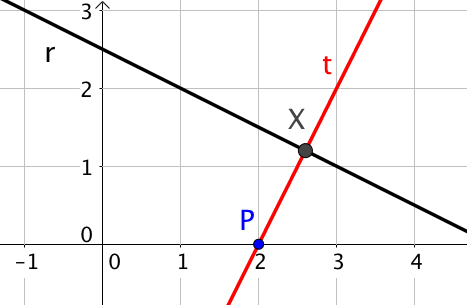
\includegraphics[width=0.4\textwidth]{img-sol/t9-12}}
	
\exer  Calculau el punt simètric de $P(6,3)$ respecte la recta $r:$ $x+2y-2=0$.

\answers{$M(4,-1)$; $P'=2M-P=2(4,-1)-(6,3)=(2,-5)$\par 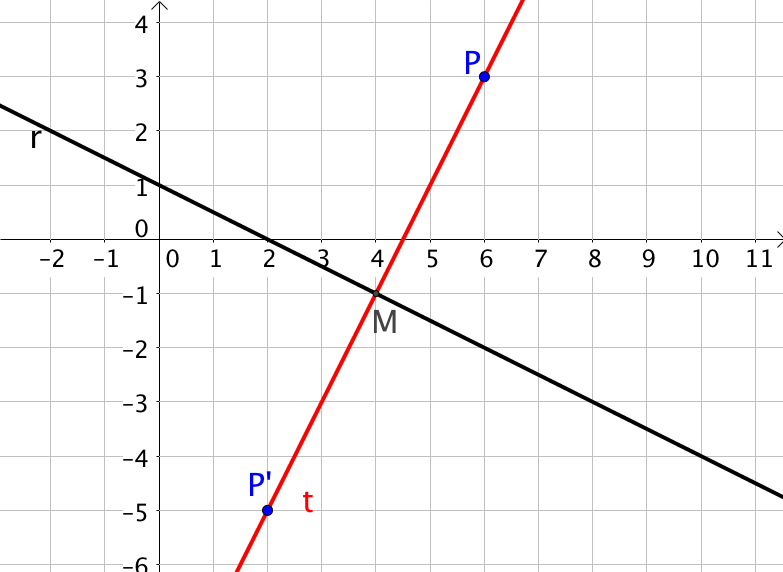
\includegraphics[width=0.4\textwidth]{img-sol/t9-13}}

\end{mylist}	

\begin{theorybox}[Feix de rectes]
    \begin{minipage}[t]{0.7\textwidth}
			Podem expressar totes les rectes que passen per un punt $P(2, 3)$ fàcilment en forma punt-pendent. En tal cas, consideram $m$ com un paràmetre.
			\[ y= 3+ m(x-2) \]
	\end{minipage}
	\begin{minipage}{0.3\textwidth}
		\centering
		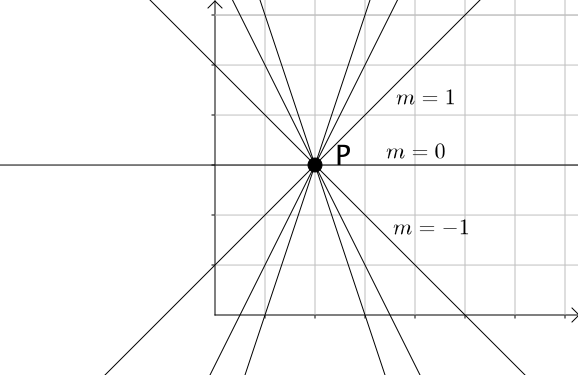
\includegraphics[width=0.8\textwidth]{img-09/feix}
	\end{minipage}
	
	

\end{theorybox}

%%%%%%%%%%%%%%%%%%%%%%%%%%%%%%%%%%%%%%%%%%%%%%%%%%%%%%%%%%%%%%%%%%%%%%%%%%%%%%%%%%%%%%%%%%%%%%%
\section{Posició relativa de dues rectes}
\begin{theorybox}[Segons punts i vectors]
	Ens donen dues rectes en el pla $r$ i $s$ de les quals sabem un punt i un vector director. La posició relativa es determina de la següent forma:
	\begin{equation}
		\vec d_r,\, \vec d_s : \left\{
		\begin{array}{l}
			\text{Diferent direcció} \rightarrow \text{Secants} \\
			\text{Igual direcció}:\left\{
			\begin{array}{l}
				R \in s \rightarrow \text{Coincidents} \\
				R \notin s \rightarrow \text{Paral·leles}
			\end{array}
			\right.
		\end{array}
		\right.
	\end{equation}
\end{theorybox}

\begin{comment}
\begin{theorybox}[Segons l'equació general]
	Donades les rectes $r: Ax+By+C=0$ i $s: A'x+B'y+C'=0$ en forma general, poden determinar la posició relativa:
	\begin{multicols}{3}
		$\dfrac{A}{A'}\neq \dfrac{B}{B'}$ 
		
		són secants.
		
		 $\dfrac{A}{A'} = \dfrac{B}{B'} \neq \dfrac{C}{C'}$ 
		 
		 són paral·leles.
		 
	 $\dfrac{A}{A'} = \dfrac{B}{B'} = \dfrac{C}{C'}$ 
	 
	 són coincidents.
	\end{multicols}
	
\end{theorybox}	
\vspace{2cm}
\end{comment}
\pagebreak

\begin{resolt}[E]{Determina la posició relativa de les rectes i el punt de tall si existeix.
\begin{equation*}
	r: \left\{ \begin{array}{l} x=1+2\lambda \\ y= 14 - \lambda \end{array}\right.
\end{equation*}	
\begin{equation*}
	s: \frac{x-2}{1}=\frac{y}{-5}
\end{equation*}	
}
Els vectors directors de les rectes $\vec d_r = (2,-1)$ i $\vec d_s = (1,-5)$ tenen clarament diferent direcció, aleshores les rectes són secants.

Per trobar el punt de tall, passam la recta $s$ a forma general $5x+y-10=0$. Tot seguit hi substituïm la $x$ i la $y$ de la recta $r$
\begin{equation*}
5(1+2\lambda)+(14-\lambda)-10=0
\end{equation*}	
Resolem aquesta equació de 1r grau i obtenim $\lambda=-1$. Si substituïm aquest valor dins la recta $r$, trobam el punt de tall $(-1,15)$.
\end{resolt}
\vspace{-0.5cm}
\begin{resolt}{Per a quin valor de $k$ les rectes 
		\begin{eqnarray*}
		r: 2x+ky-1=0 \\
		s: 3x-y+5=0
		\end{eqnarray*}	
		seran paral·leles? Hi ha algun valor pel qual siguin coincidents?}
	
	Els vectors normals de les rectes són $\vec n_r=(2,k)$ i $\vec n_s=(3,-1)$. Perquè les rectes siguin paral·leles també ho han d'ésser els seus vectors normals. Aleshores
	\begin{equation*}
	 \frac{2}{3}=\frac{k}{-1}
	\end{equation*}	
	Aïllam $k$ de l'equació i obtenim $k=-\frac{2}{3}$.
	
	Donat que 
	\begin{equation*}
	\frac{2}{3}\neq \frac{-1}{5}
	\end{equation*}	
	les rectes mai seran coincidents.
\end{resolt}
		

\begin{mylist}
	
 
	\exer  Siguin les rectes $r:\, \left\{\begin{array}{l} {x=2+\lambda } \\ {y=1-2\lambda } \end{array}\right. $ i $s:\, 2x+y=2$. Estudia la seva posició relativa i calcula els seus punts de tall si els hi hagués.
	
	\answers{$\vec d_r=(1,-2)$; $\vec d_s=(1,-2)$; $R(2,1)$; vectors paral·lels i $R\notin s$ llavors són paral·leles.}
	
	\exer  Siguin les rectes $r:\, (x,y)= \left(1,\; 1\right)+\lambda \left(-1,\; 2\right)$ i $s:\, x+y=3$. Estudia la seva posició relativa i calcula els seus punts de tall si els hi hagués.
	
	\answers{$\vec d_r=(-1,2)$; $\vec d_s=(1,-1)$; vectors independents són secants. Punt de tall $1-\lambda+1+2\lambda=3$ trobam $\lambda=1$ i el punt de tall $X(0,3)$ }
	
	\exer  Siguin les rectes $r:\, (x,y)=\left(0,\; -2\right)+\lambda \, \left(1,\; 4\right)$ i $s:\, 4x-y-2=0$. Estudia la seva posició relativa i calcula els seus punts de tall si els hi hagués. 
	
	\answers{$\vec d_r=(1,4)$; $\vec d_s=(1,4)$; $R(0,-2)$; vectors paral·lels i $R\in s$. Són coincidents. Hi ha infinits punts de tall (tots els de la recta)}
	
	\exer Troba $k$ perquè les rectes $r$ i $s$ siguin paral·leles.
	\begin{equation*}
		r: \, \frac{x-2}{3}=\frac{y}{-2} \quad\quad s:\, \frac{x+5}{-6}=\frac{y-1}{k}
	\end{equation*}
	
	\answers{$\vec d_r=(3,-2)$ i $\vec d_s=(-6,k)$. Volem que siguin paral·leles $\frac{3}{-6}=\frac{-2}{k}$, trobam $k=4$. Comprovam que efectivament són paral·leles ja que $R(2,0)$ no pertany a la recta $s$.}
	
	\exer Per a qui valor de $k$ les rectes $r$ i $s$ són coincidents?
	\begin{equation*}
		r: \, 2x+3y+5=0 \quad\quad s:\, \left\{\begin{array}{l} x=-6t+k\\ y=4t+2 \end{array}\right.
	\end{equation*}
	
	\answers{Per exemple si agafam el punt $S(k,2)$ de la recta $s$ i l'introduïm a la recta $r$ trobam $2k+6+5=0$, aleshores $k=-11/2$. Comprovam que efectivament són coincidents ja que els vectors directors $\vec d_r =(3,-2)$ i $\vec d_s=(-6,4)$ són paral·lels.}
	
	\exer Donada la recta $r:\, \left\{ \begin{array}{l}
	x=-1+3t \\
	y=2+kt
	\end{array} \right.$, troba el valor de $k$ per a què sigui paral·lela a la bisectriu del segon quadrant.

	\answers{La bisectriu del segon quadrant és $y=-x$, té pendent $m=-1$ o vector director $\vec d_s(1,-1)$. D'altra banda, la recta $r$ té vector $\vec d_r (3,k)$. Imposam que siguin paral·lels, $\frac{1}{3}=\frac{-1}{k}$ i trobam $k=-3$ }
\end{mylist}	

	
\pagebreak
%%%%%%%%%%%%%%%%%%%%%%%%%%%%%%%%%%%%%%%%%%%%%%%%%%%%%%%%%%%%%%%%%%%%%%%%%%%%%%%%%%%%%%%%%%%	
\section{Distàncies}
\begin{theorybox}
	\textbf{Distància entre dos punts}: És igual al mòdul del vector que els uneix 
	\begin{equation*}
		d(A,B)=|\overrightarrow{AB}|=\sqrt{(B_x-A_x)^2 + (B_y-A_y)^2}
	\end{equation*}
	
	\textbf{Distància entre un punt i una recta}: Si el punt pertany a la recta la distància és zero. En cas contrari, suposem que la recta ve donada en forma general $Ax+By+C=0$. Aleshores, la distància s'obté de:
	\begin{equation*}
	d(P,r)=\frac{|A\,P_x+B\,P_y+C|}{\sqrt{A^2+B^2}} 
	\end{equation*}
	
\textbf{Distància entre dues rectes}: Si les dues rectes són secants o coincidents la distància és zero. Si les rectes són paral·leles basta en calcular la distància d'un punt qualsevol de la recta $s$ a la recta $r$.
\end{theorybox}

 \begin{theorybox}[Angle entre rectes]
 	Per calcular l'angle que formen dues rectes $r$ i $s$ basta calcular l'angle que formen els seus vectors directors (o vectors normals). Per això utilitzam l'equació (\ref{eq:angle})
  \begin{equation*}
 \alpha = \arccos \dfrac{\vec d_r \cdot \vec d_s}{|\vec d_r|\, |\vec d_s|}
 \end{equation*}
 \end{theorybox}

\begin{resolt}[E]{Per a quins valors de $k$ els punts $P(10,4)$ i $Q(1,k)$ es troben a distància 15 unitats?}
	La fórmula de la distància entre dos punts
	\begin{equation*}
	dist(P,Q)=\sqrt{(1-10)^2+(k-4)^2}=15
	\end{equation*}
	Si elevam al quadrat per eliminar l'arrel, arribam a l'equació de segon grau $81+(k-4)^2=225$ que té com a solucions $k=-8$ i $k=16$.
\end{resolt}
\begin{resolt}{Calcula el punts sobre la recta $y=2x$ que distin 1 del punt $P(1,1)$.}
	Passam la recta a forma vectorial $(x,y)=(\lambda, 2\lambda)$. La fórmula de la distància entre dos punts
	\begin{equation*}
		dist(X,P)=\sqrt{(\lambda-1)^2+(2\lambda-1)^2}=1
	\end{equation*}
	Elevam al quadrat l'equació arribam a $5\lambda^2-6\lambda+1=0$. Aquesta equació de segon grau té dues solucions $\lambda=1$ i $\lambda=1/5$. Substituint cada valor de $\lambda$ dins la forma vectorial, trobam els punts de la recta $X_1=(1,2)$ i $X_2=(\frac{1}{5}, \frac{2}{5})$.
\end{resolt}

\pagebreak

\begin{resolt}{Calcula l'àrea del triangle de vèrtexs $A(-3,-2)$, $B(9, 7)$ i $C(2,8)$.
		
	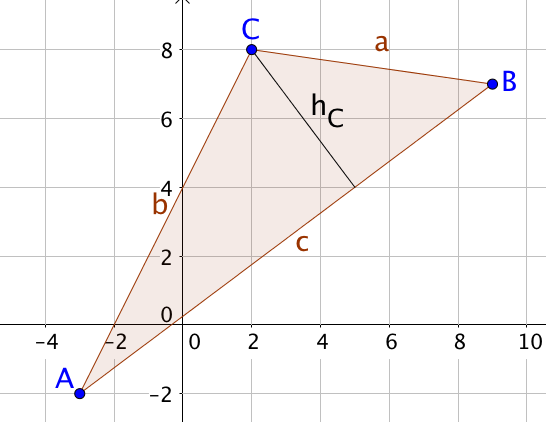
\includegraphics[width=5cm]{img-09/chap-anal-areat}
	}
	Necessitam calcular l'altura $h_C$. Per això, hem d'obtenir l'equació de la recta que passa per $A$ i $B$:\vspace{0.25cm}
	
	Pendent: $m=\frac{9}{12}=\frac{3}{4}$ $\rightarrow$ $y+2=\frac{3}{4}(x+3)$ $\rightarrow$ \fbox{$3x-4y+1=0$}\vspace{0.25cm}
	
	Altura: $h_c=dist(C, r_{AB})=\dfrac{|3\cdot 2-4\cdot 8+1|}{\sqrt{3^2+4^2}}=\frac{25}{5}=5$.\vspace{0.25cm}
	
	La base $c=dist(AB)=\sqrt{(9+3)^2+(7+2)^2}=15$\vspace{0.25cm}
	
	Àrea del triangle: $A=\dfrac{15\cdot 5}{2}=37.5\, u^2$
\end{resolt}
\begin{resolt}{Troba un punt de l'eix de les abscisses que equidisti de les rectes $4x+3y+6=0$ i $3x+4y-9=0$.}
	
	Si el punt es troba l'eix de les abscisses serà de la forma $P(x,0)$. \vspace{0.25cm}
	
 	Distància de $P$ a la 1a recta: $d_1 = \dfrac{|4x+6|}{\sqrt{4^2+3^2}}$\vspace{0.25cm}
 	
 	 Distància de $P$ a la 2a recta: $d_2 = \dfrac{|3x-9|}{\sqrt{3^2+2^2}}$\vspace{0.25cm}
	
	Igualam les distàncies: $\dfrac{|4x+6|}{5}=\dfrac{|3x-9|}{5}$ \vspace{0.25cm}
	
	Aquesta equació amb valors absoluts té dues posibilitats $4x+6=3x-9$ o $4x+6=-(3x-9)$. Cada cas dóna una solució $x=-15$ i $x=3/7$. 
\end{resolt}

\begin{mylist}
\exer   Calcula la distància del punt (1, 2) a les rectes que s'indiquen.
	\begin{tasks}(2)
		\task $x+3y=4$   \task $\left\{\begin{array}{l} {x=1-\lambda } \\ {y=2+2\lambda } \end{array}\right. $  \task $\dfrac{x-1}{2} =\dfrac{y-3}{-1} $  \task $y-2=4\left(x+1\right)$
	\end{tasks}

\answers[cols=1]{[$r:\,x+3y-4=0$; $d=\frac{3}{\sqrt{10}}$,
	$r:\,2x+y-4=0$; $d=0$,
	$r:\,x+2y-7=0$; $d=\frac{3}{\sqrt{5}}$,
	$r:\,4x-y+6=0$; $d=0$ 
	]}

\exer  Troba la posició relativa de les rectes $r{\rm :}\dfrac{x}{-{\rm 1}} =\dfrac{y+{\rm 3}}{-{\rm 1}} $ i
$s{\rm :}\left(x,y\right)=\left({\rm 1,}\; -{\rm 2}\right)+\lambda \left({\rm 1,}\; {\rm 1}\right)$
així com l'angle que formen.
\answers{$\vec d_r=(-1,-1)$; $\vec d_s=(1,1)$; $S(1,-2)$; vectors paral·lels i $S\in s$. Formen un angle de $0^\circ$ }


\exer  Tres punts d'un triangle són  \textit{A} = (2, 1), \textit{B} = (2, 8) i \textit{C} = (4, $-$1). Calculau els seus costats i angles. 

\answers{\mbox{}\par 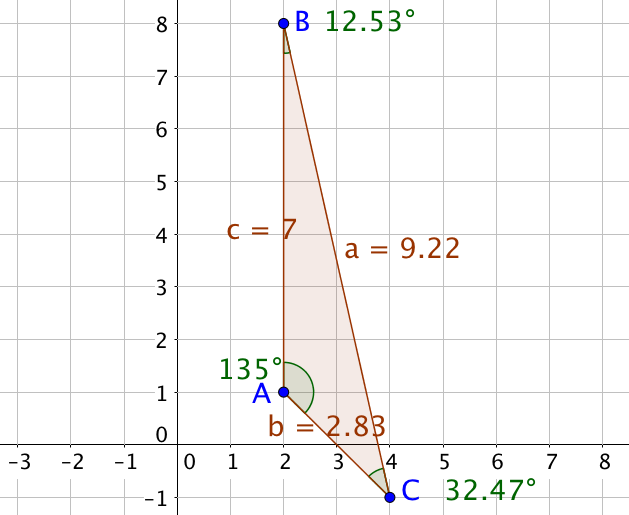
\includegraphics[width=0.4\textwidth]{img-sol/t9-21}}

\exer Determina el punt de la recta $3x-4y+8=0$ que equidista de $A(-6,0)$ i $B(0,-6)$.

\answers{La recta en forma vectorial $X:\; (x,y)=(0,2)+t(4,3)$. Imposam que les distàncies $A--X$ i $B--X$ siguin iguals: $(4t+6)^2+(2+3t)^2=(4t)^2+(3t+8)^2$. Té solució única $t=2$. Llavors el punt $X(8, 8)$.}

\exer[-1] De totes les rectes que passen pel punt $A(1,2)$ troba el pendent d'aquella que dista 1 de l'origen.
\answers{El feix de rectes és $r:$ $y-2=m(x-1)$. Passa-la a forma general i aplica que $d(r,O)=1$.}



\end{mylist}
\pagebreak

\subsection{Rectes i punts notables d'un triangle}

\begin{theorybox}
	
	Considerau el costat AB d'un triangle de vèrtexs ABC:
	
	\begin{itemize}
		\item \textbf{Mediana}: És la recta que passa pel punt mitjà $M=\frac{A+B}{2}$ del segment i que passa pel vèrtex oposat $C$.
		
		\item \textbf{Altura}: És la recta que passa pel vèrtex oposat $C$ i que és perpendicular al segment $AB$.
		
		\item \textbf{Mediatriu}: És la recta que passa pel punt mitjà de $AB$ i que és perpendicular a ell.
		
		\item \textbf{Bisectriu}: Si $r_{AB}$ és la recta que passa per $AB$ i $r_{AC}$ la recta que passa per $AC$, la bisectriu és el lloc geomètric de tots els punts $X(x,y)$ que equidisten de les dues rectes.
		\begin{equation*}
		dist(X,r_{AB}) = dist(X,r_{AC})
		\end{equation*}
	\end{itemize}
	
	
	\begin{center}
		
		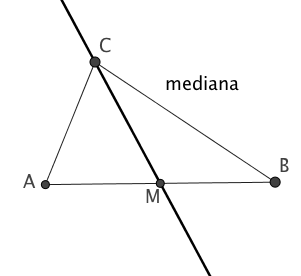
\includegraphics[height=3.cm]{img-09/mediana.png}
		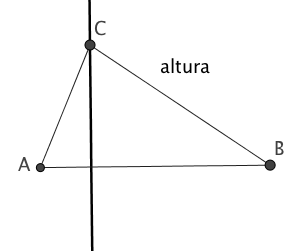
\includegraphics[height=3.cm]{img-09/altura.png}
		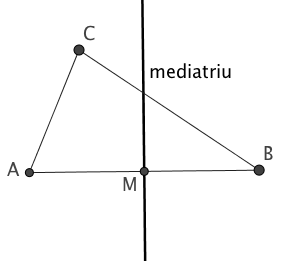
\includegraphics[height=3.cm]{img-09/mediatriu.png}
		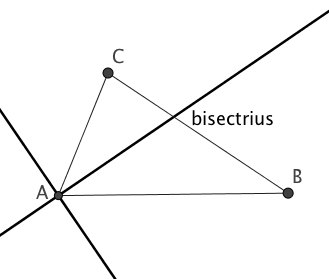
\includegraphics[height=3.cm]{img-09/bisectriu.png}
		
	\end{center}
\end{theorybox}


\begin{theorybox}[Punts notables]
	Considerau un triangle de vèrtexs ABC:
	
	\begin{itemize}
		\item \textbf{Baricentre (G)}: és el punt on es tallen les medianes. Representa el centre de gravetat del triangle.
		\item \textbf{Ortocentre (H)}: és el punt on es tallen les altures. 
		\item \textbf{Circumcentre (O)}:  és el punt on es tallen les mediatrius. És el centre de la circumferència circumscrita en el triangle.
		\item \textbf{Incentre (I)}: és el punt on es tallen les bisectrius. És el centre de la circumferència inscrita en el triangle.
	\end{itemize}
	\begin{center}
		
		
		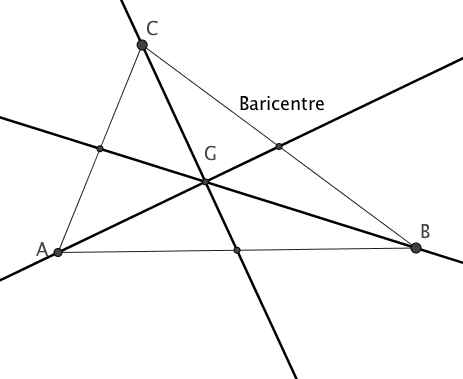
\includegraphics[height=3.cm]{img-09/baricentre.png}
		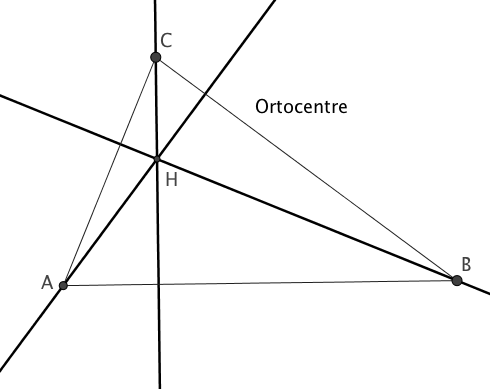
\includegraphics[height=3.cm]{img-09/ortocentre.png}
		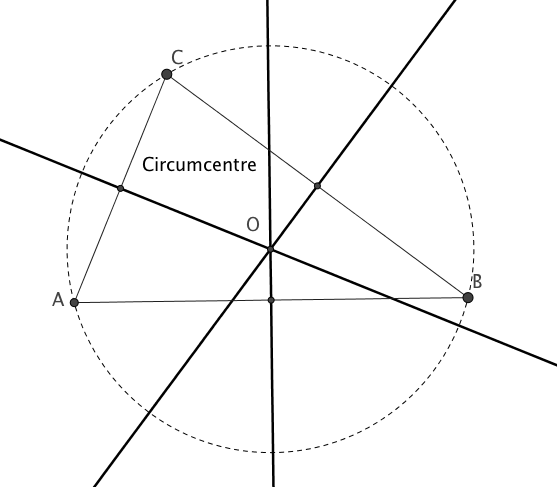
\includegraphics[height=3.cm]{img-09/circumcentre.png}
		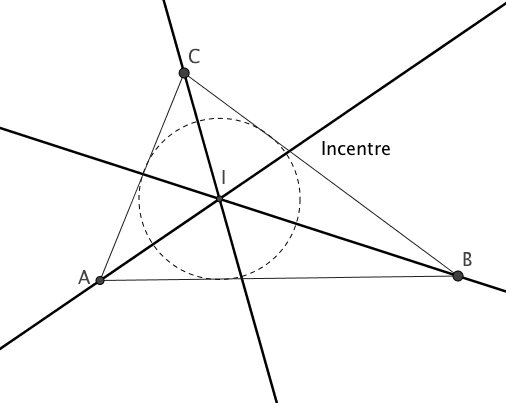
\includegraphics[height=3.cm]{img-09/incentre.png}
		
	\end{center}
	
\end{theorybox}

\begin{mylist}
			
	\exer  \hot Donat el triangle de vèrtexs \textit{ABC}, essent \textit{A} = (0, 0), \textit{B} = (6, 0) i \textit{C} = (4, 4), determina les equacions de:
	\begin{tasks}
		\task  Les seves mediatrius i les coordenades del circumcentre
		%
		\task  Les seves bisectrius i les coordenades de l'incentre
		%
		\task  Les seves altures i les coordenades de l'ortocentre
		%
		\task  Les seves medianes i les coordenades del baricentre
	\end{tasks}

\answers{\mbox{}\par 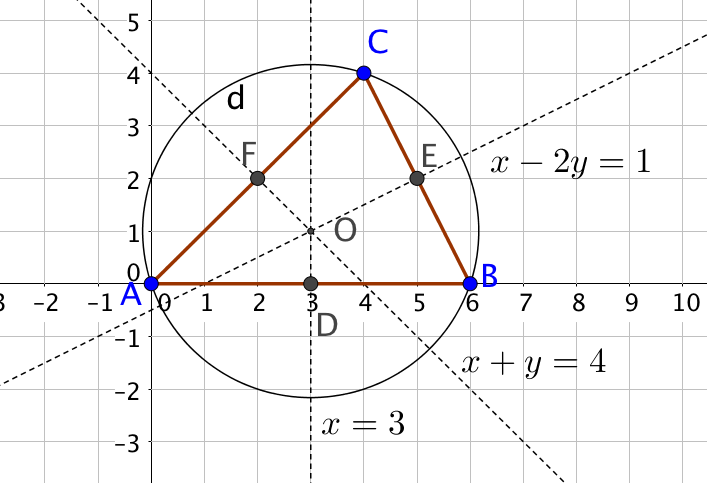
\includegraphics[width=0.4\textwidth]{img-sol/t9-22a}
\par 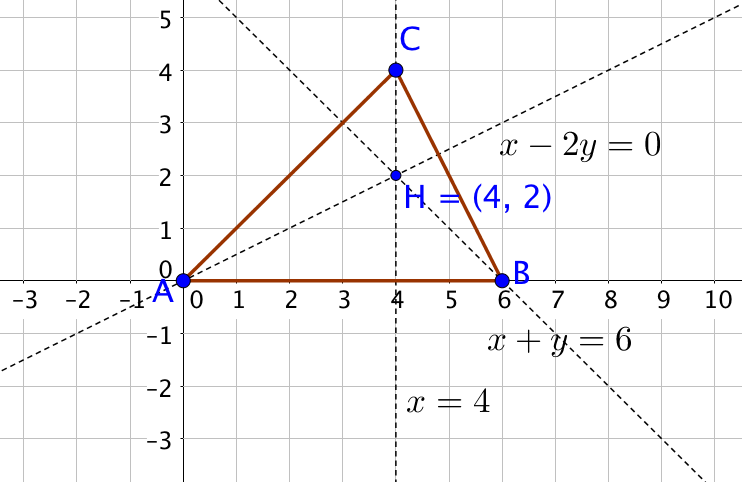
\includegraphics[width=0.4\textwidth]{img-sol/t9-22b}
\par 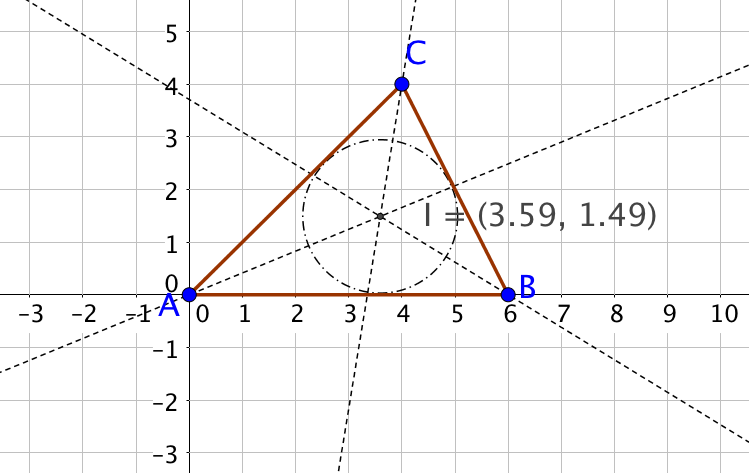
\includegraphics[width=0.4\textwidth]{img-sol/t9-22c}
\par 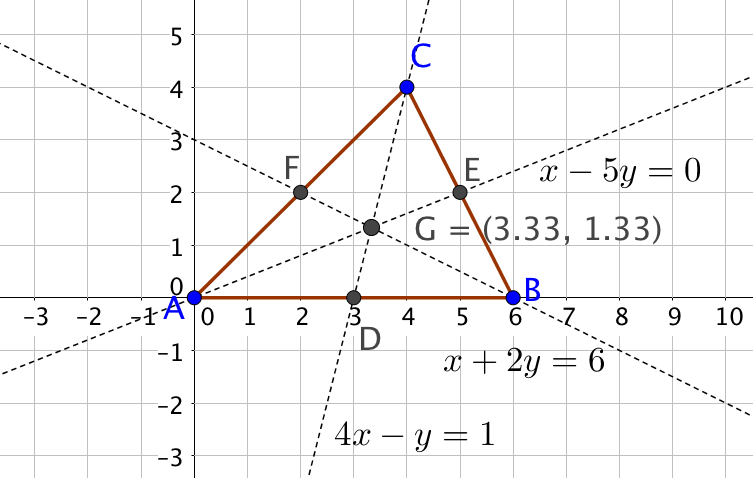
\includegraphics[width=0.4\textwidth]{img-sol/t9-22d}}
\end{mylist}


%%%%%%%%%%%%%%%%%%%%%%%%%%%%%%%%%%%%%%%%%%%%%%%%%%%%%%%%%%%%%%%%%%%%%%%%%%%%%%%%%%%%%%%%%%%%%%%%%%%%%%%%%%%%
\newpage	
\begin{activitats}
	
	\begin{mylist}	
		
		\exer  Considerem la recta  $r:\,  \frac{x-1}{-1} =\frac{y-2}{3} $. 
	
	\begin{tasks}
		\task  Calcula el seu pendent.
		%
		\task  Pertany el punt $\left(0,\, \, 5\right)$ a la recta? I el $\left(1,\; 3\right)$?
		%
		\task  Dóna almenys tres punts de la recta.
		%
		\task  Dibuixa la recta.
	\end{tasks}

\answers{[$m=-3$, $(0,5)\in r$; $(1,3)\notin r$, $(x,y)=(1,2)+\lambda(-1,3)$,
	Gràfic]}
	
	\exer  Siguin els punts \textit{A}= (1, 2) i \textit{B} = (3, 0)
	\begin{tasks}
		\task  Calcula el vector que els uneix.
		%
		\task  Calcula l'equació general de la recta que passa per tots dos.
		%
		\task  Pertany el punt (2, 1) a la recta?, i el (3, 1)?
	\end{tasks}
		
		\answers{[$\overrightarrow{AB}=(2,-2)$, $\frac{x-1}{2}=\frac{y-2}{-2}$, $(2,1)\in r$; $(3,1)\notin r$]}
		
			
		\exer  Considerem la recta $y-2x=1$
		
		\begin{tasks}
			\task  Calculau el seu pendent i vector director.
			\task  Donau una recta perpendicular a ella que passi per (1, 2). Expressa-la almenys de quatre formes.
		\end{tasks}
		
		\answers{[$m=2$; $\vec d =(1,2)$, $\frac{x-1}{-2}=\frac{y-2}{1}$]}
		
		\exer  Sigui la recta $r:\,  y=x-2$.
		
		\begin{tasks}
			\task  Calcula una recta perpendicular a ella i passi per (2, 1).
			\task  Calcula una recta que passi per (--1, 3) i sigui paral·lela a  $r$.
		\end{tasks}
	
	\answers{[$y=-x+3$, $y=x+4$]}
		
		\exer  Troba la posició relativa de les rectes $x+y=0$ i $s:\,  \left(x,y\right)=\left(1,\; 2\right)+\lambda \left(1,\, \; 1\right)$ així com l'angle que formen.
		
		\answers{Són secants formen un angle de $90^\circ$. Es tallen al punt $(-\frac{1}{2},\frac{1}{2})$}
		
		\exer  Suposa que la distància d'un punt a una recta és 0. Què significa aquest resultat? Aplica-ho a la recta $2x-y=1$ i el punt (2, 3).
		
		\answers{Si la distància $d(r, P)=0$ vol dir que el punt $P$ pertany a la recta $r$. \par Donat que $P(2,3)$ pertany a $2x-y-1=0$, podem comprovar que $d(P, r)=\frac{|2\cdot 2 - 3 -1|}{\sqrt{2^2+1^2}}=0$}
		
		\exer  Sigui la recta $s:\, x+y=4$. 
		\begin{tasks}
			\task  Calcula una recta perpendicular amb ella i passi per (1, 1). 
			\task  Calcula la distància d'aquesta recta al punt (2, 3).
		\end{tasks}
	
		\answers[cols=1]{[$y=x$, $d=\dfrac{|2-3|}{\sqrt{1^2+1^2}}=\frac{\sqrt{2}}{2}$]}

	
	\exer  Sigui la recta $s:\; x-2y+1=0$ 
	
	\begin{tasks}
		\task  Calcula una recta que sigui perpendicular a ella i passi per (1, 1).
		\task  Calcula una recta que passi per (0, 1) i sigui paral·lela a  $s$.
	\end{tasks}
	
	\answers{[$2x+y+3=0$, $x-2y+2=0$]}

	\exer  Tres punts d'un rectangle \textit{ABCD} són \linebreak \textit{A} = (2, 1), \textit{B}= (0, 7) i \textit{D} = (5, 2). Es demana:
	\begin{tasks}
		\task  Calcular el punt \textit{C}.
		%		
		\task  Comprovar que l'angle \textit{B} és de 90º.
		%
		\task  Calcular les longituds dels costats \textit{AB}, \textit{BD} i \textit{CD} del rectangle.
	\end{tasks}

\answers[cols=1]{[$C(3,8)$, $\overrightarrow{BC}=(3,1)$ i $\overrightarrow{BA}=(2,-6)$. Es compleix que $(3,1)\cdot(2,-6)=0$ són perpendiculars, 
	$\overline{AB}=2\sqrt{10}$; $\overline{BD}=5\sqrt{2}$; $\overline{CD}=\overline{AB}=2\sqrt{10}$]}
	
		
		\exer  Troba la posició relativa de les rectes $r:\, 3x+y=5$ i $s:\, \left(x,y\right)=\left(1,-2\right)+\lambda \left(-1,3\right)$ així com l'angle que formen.
		
		\answers{Són paral·leles, formen un angle de $0^\circ$}
		
		\exer  Calcula la recta perpendicular a \linebreak $y=2x-4$  que passi pel punt mitjà de \textit{A} = (1, 3) i \textit{B} = (3,-1)
		
		\answers{$M=(2,1)$; $y=-\frac{1}{2}x+2$}
		
		\exer  Calcula la distància a l'origen de les rectes que s'indiquen.
		\begin{tasks}(2) 
			\task $2x+y=3$  \task  $y=\dfrac{x}{2} $ \task*(2)  $\left(x,y\right)=\left(1,\; -2\right)+\lambda (1,1) $ 
		\end{tasks}
		
		\answers{[$d(O,r)=\frac{3\sqrt{5}}{5}$, $d(O,r)=0$, $d(O,r)=\frac{3\sqrt{2}}{2}$]}
	
		\exer  Calcula la distància del punt (2, $-$1) a la recta $y+x=1$. 
		
		\answers{La distància és zero, perquè el punt pertany a la recta.}
		
		\exer  Calcula la distància al punt (1, $-$2) de les següents rectes.
		\begin{tasks}(2)
			\task $\left\{\begin{array}{l} {x=1+\lambda } \\ {y=-\lambda } \end{array}\right. $   \task $2x+y=3$ 
		\end{tasks}
		
		\answers{[$r:\;x+y-1=0$; $d(P,r)=\frac{\sqrt{2}}{2}$, $d(P,r)=\frac{3\sqrt{5}}{5}$]}
		
		\exer  Calcula la distància del punt (1, 4) a la recta $y-x=1$ 
		\answers{$d(P,r)=\sqrt{2}$}
		
		
		\exer[-1]  Una recta passa pel punt (3, 1) i forma amb els semieixos positius un triangle d'àrea 6 unitats. Calcula l'equació d'aquesta recta.
		
		\answers{Escriu el feix de rectes com $y=1-m(x-3)$, troba els punts de tall amb els eixos i comprova que l'àrea és $A=\frac{1}{2}(1+3m)(3+\frac{1}{m})=6$. Resol l'equació i troba $m=1/3$.}
		
		\exer  Calcula el punt de simètric de $A=(1, 2)$ respecte a la recta $y=3$.
		
		\answers{Gràficament $A'(1,4)$}
		
		\exer  Considerem un pentàgon irregular \textit{ABCDE} format pels punts 
		\textit{A} =($-$2, 3),  \textit{B} = (1, 4), \textit{C}= (3,3), \textit{D} = (2, 2) i \linebreak \textit{E} = ($-$1, 1). 
		Dibuixa-ho i calcula la seva àrea.  Et recomanem dividir-ho en figures més manejables.
		
		\answers{\mbox{}\par 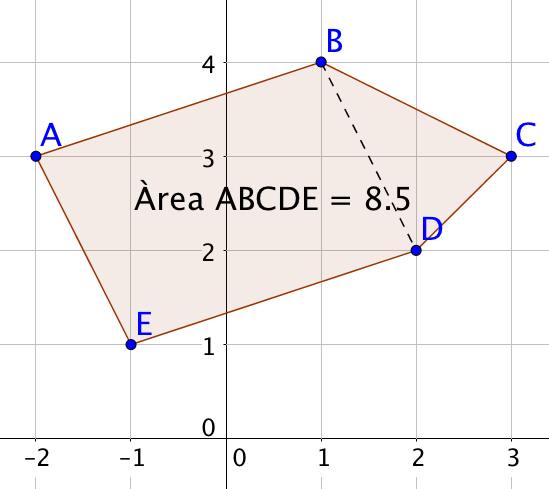
\includegraphics[width=0.4\textwidth]{img-sol/t9-40}}
		
		\exer[-1]  Considerem un quadrat \textit{ABCD}. El punt \textit{A} és (1, 2) i els punts \textit{B} i \textit{C} estan sobre la recta $r:\, y-x=3$. Calcula els quatre vèrtexs del quadrat i la seva àrea.
		\answers{Troba el peu de la perpendicular de $r$ pel punt $A$: $B=(0,3)$, $C=(1,4)$ i $D=(2,3)$ }
		
		
		\exer  Determina les mediatrius dels segments d'extrems \textit{A} i \textit{B}. Representa-ho gràficament.
		\begin{tasks}
			\task \textit{A =} (0, 7) i \textit{B} = (0, 3)   \task \textit{A =} (--3, 0) i \textit{B} = (6, 0)   \task\textit{A =} (--5, 0) i \textit{B} = (0, --5)
		\end{tasks}
	
		\answers{[$y=5$, $x=\frac{9}{2}$, $y=x$ ]}
		
		\exer  Determina les bisectrius de les rectes $r$ i $s$ per cada un dels casos següents. Representa-ho gràficament.
		\begin{tasks}
			\task $r: \, x+2y-5=0$ i
			
			 $s: \, 2x-y-8=0$
			\task $r: \, 3x+5y-2=0$ i 
			
			$s: \, 4x-6y-1=0$
			\task $r: \, x=0$ i $s: \,y=0$
			\task $r: \, x+y=0$ i $s: \, x-y=0$
		\end{tasks}
		 
		 \answers{[$y=-3x+13$ i $y=\frac{1}{3}x-1$,
		 	$y=-42.02x+18.93$ i $y=0.02x+0.12$,
		 	$y=x$ i $y=-x$,
		 	$x=0$ i $y=0$]}
	
		\exer  Considera la recta $x+2y=3$ i el punt $A(2, 3)$. Calcula el punt \textit{Q} de mínima distància i el simètric de  \textit{A} respecte de la recta.
		
		\answers{La perpendicular $2x-y=1$, $Q(1,1)$ i el simètric $A'(0,-1)$}
	
		\exer  En un paral·lelogram \textit{ABCD}, els vèrtexs venen donats per \textit{A} = (1, 1), \textit{B}= (2, 3) i \textit{C}= (3, $-$1).
		\begin{tasks}
			\task  Calcula l'angle $\hat B$ (entre els costats \textit{BA} i \textit{BC}).
			%
			\task  Calcula l'equació de la recta que passa per \textit{A} i \textit{C} (la diagonal del paral·lelogram).
		%			
			\task  Calcula el perímetre de la figura.
		%	
			\task  Calcula el punt \textit{D}.
		\end{tasks}
	
		\answers{Perímetre: 10.14\par 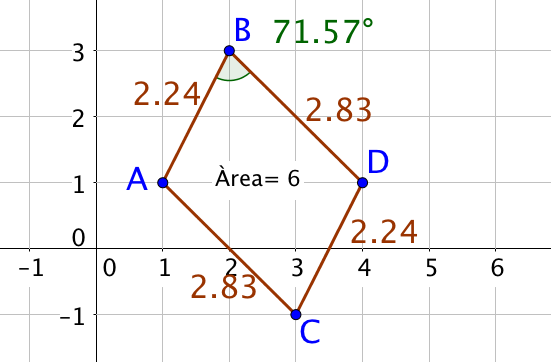
\includegraphics[width=0.4\textwidth]{img-sol/t9-45}}
		
		\exer  La recta $2x+y-4=0$ és la mediatriu d'un segment que té un extrem al punt (0, 0). Troba les coordenades de l'altre extrem.
		
		\answers{L'altre extrem del segment és el simètric de $O$ respecte r. 
		$O'(\frac{16}{5}, \frac{8}{5})$}
		
	\exer  Recordem que el circumcentre d'un triangle és el punt de tall de les mediatrius dels seus costats. Calcula el circumcentre del triangle \textit{A =} (1, 2), \linebreak \textit{B} = (1, 6) i \textit{C} = (3, 8) escrivint les equacions de les tres mediatrius.
		
	\answers{\mbox{}\par 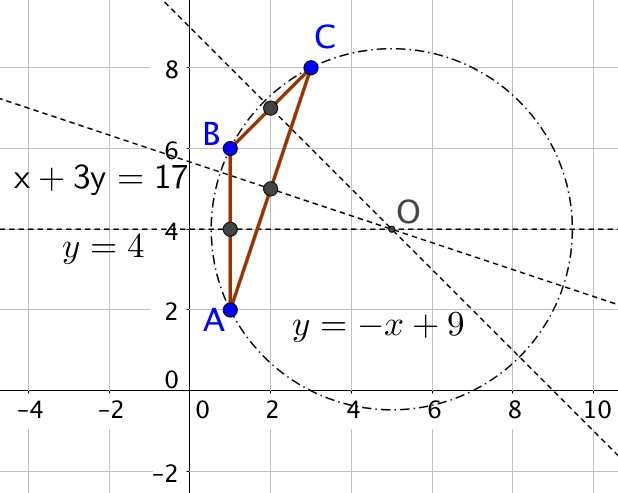
\includegraphics[width=0.4\textwidth]{img-sol/t9-47}}
	
	
	\exer  El baricentre d'un triangle és el punt d'intersecció de les medianes (la mitjana és la recta que va des d'un vèrtex al punt mitjà del costat oposat). Sabent això, calcula el baricentre del triangle \textit{A}=($-$2, 2), \textit{B}=(1, 4) i \textit{C} = (1, 0), escrivint les equacions de les tres medianes.
		
	\answers{\mbox{}\par 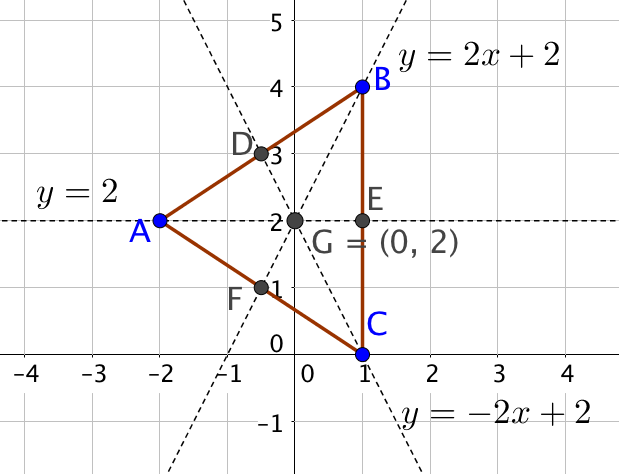
\includegraphics[width=0.4\textwidth]{img-sol/t9-48}}
			
	\exer  La recta $x+y-2=0$ i una recta paral·lela a ella que passa pel punt (0, 5) determinen, juntament amb els eixos de coordenades, un trapezi isòsceles. Troba'n l'àrea.

	\answers{$A=\frac{21}{2}$.\par 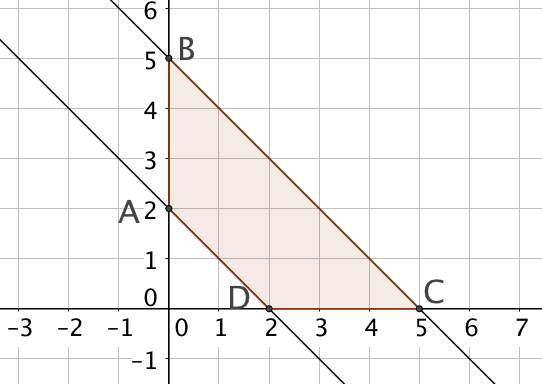
\includegraphics[width=0.4\textwidth]{img-sol/t9-trapz}}
	
	\exer Troba el punt de l'eix de les abscisses que equidisti de les rectes $r:\, 4x+3y+6=0$ i $s:\, 3x+4y-9=0$.
	
	\answers{El punt és $X(x,0)$. S'ha de complir que $\dfrac{|4x+6|}{5}=\dfrac{3x-9}{5}$. Trobam dues equacions $4x+6=\pm (3x-9)$. Té dues solucions $x=-15$ i $x=\frac{3}{7}$}
	
\end{mylist}	
	
\end{activitats}	

\newpage


\begin{resolt}[E]{Troba el les altures i l'ortocentre del triangle amb vèrtexs $A(2,0)$, $B(0,1)$ i $C(-3,-2)$.
	
\begin{center}	
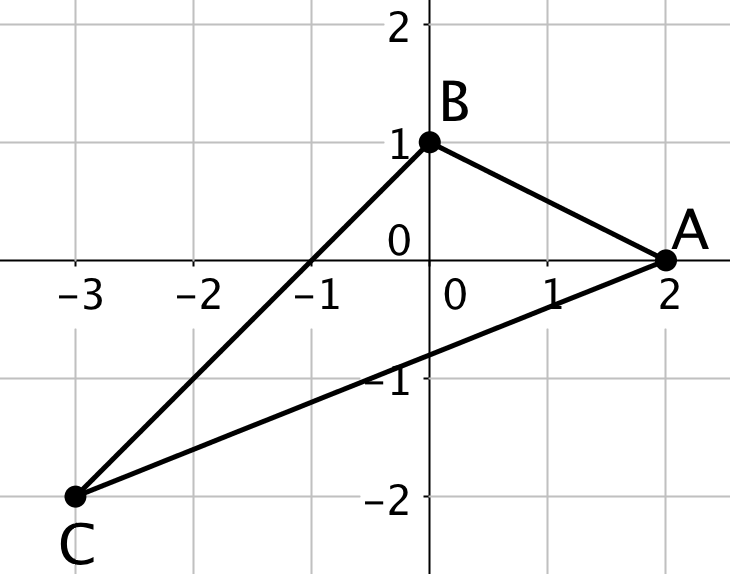
\includegraphics[width=0.25\textwidth]{img-09/triangle-ortocentre}
\end{center}
}
	
	$h_C$: Altura que parteix de $C$ i es perpendicular a AB \vspace{0.25cm}
	
	$m_{AB}=-\frac{1}{2}$; \; $m_{h_C}=2$:\; $y=-2+3(x+3)$ \; $\rightarrow$\;  $2x-y+4=0$\vspace{0.35cm}


	
	$h_B$: Altura que parteix de $B$ i es perpendicular a AC\vspace{0.25cm}

	$m_{AC}=\frac{2}{5}$; \; $m_{h_C}=-\frac{5}{2}$:\; $y=1-\frac{5}{2}x$ \; $\rightarrow$\;  $5x+2y-2=0$\vspace{0.35cm}

	L'ortocentre s'obté del punt d'intersecció de les altures\vspace{0.25cm}
	
	$\left. \begin{array}{l} 2x-y+4=0 \\  5x+2y-2=0 \end{array} \right\}$ \;  $\rightarrow$ \; $\boxed{H=\left(-\frac{2}{3}, \frac{8}{3}\right)}$\vspace{0.25cm}

\end{resolt}

\vspace*{\fill}

\begin{autoaval}{31}
\begin{mylist}
	\exer[2] Es consideren els punts $A(0,1)$, $B(4,9)$ i $C(-4,k)$. Troba $k$ perquè
	\begin{tasks}
		\task Els punts estiguin alineats.
		\task Perquè el punt $C$ sigui el punt simètric de $B$ respecte $A$.
	\end{tasks}
	\answers{ a) $k=-7$, b) $k=-7$}

	\exer[2] Calcula l'equació de les rectes:
		\begin{tasks}
		\task Que passa per $A(3,2)$ i $B(-2,1)$ en forma contínua i general.
		\task Que passa per $A(1,1)$ i té pendent $-3$ en forma punt-pendent i general.
	\end{tasks}
	\answers{Contínua $\frac{x-3}{5}=\frac{y-2}{1}$, general $x-5y+7=0$.}
	
	\exer[2] Calcula l'equació de les rectes:
	\begin{tasks}
		\task Passa per $P(2,-3)$ i és perpendicular a $(x,y)=(0,1)+t(5,-2)$.
		\task És paral·lela a $2x+3y+1=0$ i passa pel punt $(0,2)$.
	\end{tasks}
	\answers{a) $(x,y)=(2,-3)+\lambda(2, 5)$,  b) $2x+3y-6=0$.}
	
	\exer[2] Estudia la posició relativa de les rectes $r$ i $s$ segons els valors del paràmetre $k$
  	$r: \, 3x+ky-34=0$ i $s: \, y=\frac{5}{3}x$.	
	 \answers{Si $k=-9/5$ són paral·leles, en altre cas són secants.}

	\exer[2]  Calcula $k$ perquè les rectes $y=3$ i $y=kx+1$ formin un angle de $60^\circ$.
	\answers{$k=\pm \sqrt{3}$.}
	
	\exer[2] Troba tots els punts situats sobre la recta $y=2x+1$ que es troben a distància $\sqrt{52}$ del punt $A(1,1)$.
	\answers{$x=-3$, $y=-5$ i $x=17/5$ i $y=39/5$}
\end{mylist}
\end{autoaval}

\vspace*{\fill}